% This file should be replaced with your file with thesis content.
%=========================================================================
% Authors: Michal Bidlo, Bohuslav Křena, Jaroslav Dytrych, Petr Veigend and Adam Herout 2019

% For compilation piecewise (see projekt.tex), it is necessary to uncomment it and change
% \documentclass[../projekt.tex]{subfiles}
% \begin{document}

\chapter{Note to the Reader}
Through the thesis, the expression "iff" refers to "if and only if".\\
Except if explicitely stated otherwise, the following notation conventions apply throughout the thesis. 
In the context of regular languages, lower case latin alphabet letters, such as $a, b, c, \dots$, reffer to terminal symbols. Upper case latin alphabet letters, such as $A, B, C,\dots$, denote nonternminal symbols.

\chapter{Introduction}
\todo{Add motivation for thesis, talk about importance of optics simulations, talk about uses, show examples. Talk about the need to compare simulation software.}

\chapter{Review of Relevant Literature}
This chapter aims to give the reader a broad understanding of the subjects of matter. It provides an overview of the physics behind the aforementioned simulations and an introduction to the basic concepts of compiler design and the underlying formal language theory. This chapter will not delve into the specifics of each subject at hand but will provide the reader with the foundations necessary to comprehend the rest of this thesis.

\section{Computational Electromagnetics}
\subsection*{Curl theorem}
\subsection*{Divergence theorem}
\subsection*{Maxwell's equations}
\todo{show all 4 equations}
\todo{derive partial form form integral form}



\subsection*{Finite Difference Time Domain}
\section{Formal Language Theory}
We use languages like English or Slovak every day to communicate information, these languages are referred to as \emph{natural languages}. The Oxford English Dictionary defines language as a system of spoken or written communication used by a particular country, people, community. How ever a more rigorous definition of languages and the tools to operate on them is required. That is what the notion of formal language theory will introduce in the following sections.

\subsection{Alphabets and Languages}

\todo{add text about languages and alphabets, use English as example}

\begin{definition}[Alphabet]
\label{def:alphabet}
Let $\Sigma$ be an \emph{alphabet}, a finite nonempty set of symbols, letters. Then $\Sigma ^{*}$ defines the set of all sequences $w$:
$$w= a_1 a_2 a_3 \dots a_{n-1} a_n, \in \Sigma \text{ for } n \in \mathbb{N}$$
\end{definition}

The sequence of symbols $w$ is called a \emph{word}. The length of a word is given by the number of symbols $a$, symbolically $|w| = n$. The word with a length of 0 is called an \emph{empty word} denoted as $\epsilon$.

\begin{definition}[Language]
\label{def:language}
The set $L$ where $L\subseteq \Sigma^{*}$ is know as the \emph{formal language} over the alphabet $\Sigma$. 
\end{definition}
The words $L = \left\lbrace \epsilon, a, b, aa, ab, bb \right\rbrace$ are some words of a language $L$ over the alphabet $\Sigma=\left\lbrace a,b \right\rbrace$.
Other examples for languages over the alphabet $\Sigma=\left\lbrace a,b \right\rbrace$ might include:
\begin{itemize}
\item $L_1 = \left\lbrace \epsilon \right\rbrace$
\item $L_2 = \left\lbrace a \right\rbrace$
\item $L_3 = \left\lbrace aaa \right\rbrace$
\item $L_4 = \left\lbrace a^i,b^i; i \in \mathbb{N} \right\rbrace$
\end{itemize}




\paragraph*{Notation conventions}



\begin{itemize}
\item Iteration\\
  Let $a^i; a \in \Sigma \text{ and } i \in \mathbb{Z}$ be the \emph{iteration} of a character $a$, where $|a^i| = i$.\\
Example bellow:


\begin{itemize}
\item $a^0 = \epsilon$
\item $a^1 = a$
\item $a^2 = aa$
\item $a^i = a_0 a_1 a_2 \dots a_i; i \in \mathbb{N}$
\end{itemize}



\item Concatenation\\
  Let $w \cdot w^{'}; w, w^{'} \in \Sigma^{*}$ be the \emph{concatenation} of the words $w$ and $w^{'}$.

$w = a_1 a_2 a_3 \dots a_n ; w^{'} = a^{'}_1 a^{'}_2 a^{'}_3 \dots a^{'}_m; n,m \in \mathbb{Z}$ then  

$w\cdot w^{'} = w w^{'} = a_1 a_2 a_3 \dots a_n a^{'}_1 a^{'}_2 a^{'}_3 \dots a^{'}_m$


\item \todo{Kleene star}
\item Symbol count\\
The number of occurrences of $a$ in $w$, where $a \in \Sigma, w \in \Sigma^{*}$, noted as $|w|_{a}$.

\end{itemize}

\subsection{Grammars}
Linguists refer to grammar as a set of rules that specify how a natural language is formed. Due to the polysemous and vague nature of natural languages, it is not suited for the description of unambiguous systems. The inherit need to strictly describe languages introduced various language defining mechanisms. Many of these mechanisms are interchangeable, and may describe the same languages. How ever, not all mechanisms are able to describe languages formed by other mechanisms.

The concept of a grammar is a powerful tool for describing languages\cite[p. 52]{Linz2016Introduction}. A simple sentence in English consists of a single independent clause. A clause is typically formed by a subject and a predicate. This can be written as follows.
$$ \left< clause \right> \rightarrow \left< subject \right> \left< predicate \right> $$

We can further define the $\left< subject \right>$ and $\left< predicate \right>$. One of the possible subjects is a noun phrase, and the predicate may be a simple verb.
$$\left< subject \right>   \rightarrow   \left< determiner \right>   \left< premodifier \right>    \left< noun \right>    \left< postmodifier \right>$$
$$\left< predicate \right> \rightarrow \left< verb \right>$$

Associating the $\left< determiner \right>$ with the article "the", $\left< premodifier \right>$ with "fast" or "slow", $\left< noun \right>$ with "athlete", $\left< postmodifier \right>$ to "from England" or to an empty string and finally associating the $\left< verb \right>$ to "won" or "lost" allows us to write multiple sentences like "The fast athlete from England won" or "The slow athlete lost". These sentences are considered to be \emph{well formed}, as they resulted from following the grammatical rules.

The premise is consecutively replacing $\left< clause \right>$ until only irreducible blocks of the language remain. Generalizing this idea brings about the concept formal grammars.

\begin{definition}[Grammar]
\label{def:grammar}
\cite{Salomaa1987Formal}
Let an ordered quadruple $G$ define a grammar such that: $G=\left(N, \Sigma, P, S \right)$, where:
\begin{enumerate}
\item $N$ is a finite set of \emph{nonternminal} symbols
\item $\Sigma$ is an alphabet finite set of \emph{terminal} symbols, such that $N \cap \Sigma = \varnothing$
\item $P$ is a finite set of rewriting rules known as \emph{productions}, ordered pairs $\left( \alpha, \beta \right)$.
$P$ is a subset of the cartesian product of $\alpha = \left(N \cup \Sigma\right)^* N \left(N \cup \Sigma\right)^*$ and $\beta = \left(N \cup \Sigma\right)^*$


Productions are denoted as $\alpha \rightarrow \beta$.
If there are multiple productions with the same left hand side ($\alpha$), we can group their right hand sides ($\beta$).


$\alpha \rightarrow \beta_1, \alpha \rightarrow \beta_2$ may be written as $\alpha \rightarrow \beta_1 | \beta_2$

\item $S$ is the starting symbol of the grammar $G$, where $S \in N$
\end{enumerate}
\end{definition}

Productions $\alpha \rightarrow \beta$ symbolize, that given the words $V,W,x,y \in \left( N \cup \Sigma \right)^{*}$, the word $V$ can be rewritten as follows:
$V \Rightarrow W$ iff there are words, which satisfy the following condition, $V=x\alpha y \wedge W=x\beta y$ and $\alpha \rightarrow \beta \in P$.

\begin{definition}[Derivation]
\label{def:derivation}
$V \stackrel{*}{\Rightarrow}  W$ iff there is a finite set of words 
$$ v_0, v_1, v_2, \dots, v_z;\medskip z \in \mathbb{Z}$$
such that $v_0 = V$ and $v_z = W$ where each is rewritten from the previous word. Such a sequence of applications of productions is called a derivation.
The length of a derivation is given by $z$. 
\end{definition}

Grammars are often represented using formalisms, these formalisms often set restrictions on the left and right hand sides of productions. These restrictions further impose limits on the set of languages a grammar may produce, this is known as the \emph{expressive power} of a grammar. 

\subsection{Chomsky hierarchy}
When working with formal grammars, the need to compare their expressive power arose. Linguist Noam Chomsky introduced the now so called \emph{Chomsky hierarchy}\cite{chomsky1956three}. A set of four classes, each more expressive than the previous, see \cref{fig:chomsky-hierarchy}.



\begin{figure}[h]
  \caption{Description of Chomsky hierarchy.}
  \label{fig:chomsky-hierarchy}
  \centering
  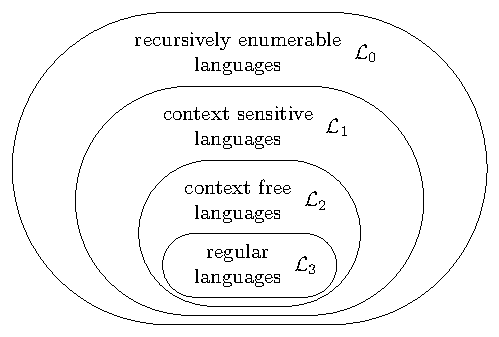
\includegraphics[width=0.75\textwidth]{figures/chomsky-hierarchy.pdf}
\end{figure}

The intricaties of each class are not necessary in the context of this thesis, how ever relugar laguages will be used heavily throughout the rest of this thesis, so they will be explained more in depth.

\begin{table}[h]
\centering
\begin{tabular}{@{}ccl@{}}
\toprule
Grammar         & Language               & Restrictions \\ \midrule
$\mathcal{L}_3$ & Regular                & \todo{todo}             \\
$\mathcal{L}_2$ & Context Free           &              \\
$\mathcal{L}_1$ & Context Sensitive      &              \\
$\mathcal{L}_0$ & Recursively Enumerable &              \\ \bottomrule
\end{tabular}
\caption{An overview of the Chomsky hierarchy classes.}
\label{tab:chomsky-hierarchy}
\end{table}

\subsection{Regular Languages}
As shown above, regular languages are the inner most part of the Chomsky hierarchy, thus they are the most constricted. How ever, regular languages play a crutial role in lexical analysis, more precisely pattern matching. These constrictions lead to many useful closure propetries and decisability properties, mainly membership, which will be introduced shortly.

Regular languges may be defined in multiple equivalent manners such as through finite automata or regular expressions. 

\subsubsection{Finite Automata}

\begin{definition}[Deterministic Finite Automata]
\label{def:dfa}
DFAs are formally defined as 5-tuples
$$ M = (Q, \Sigma, \delta, q_0, F),$$
where
$Q$ is a finite set of states. $\Sigma$ is a finite set of symbols, also know as a input alphabet. $\delta$ is a transition function between states defined as $\delta : Q \times \Sigma \rightarrow Q$. $q_0$ is a initial state, $q_0 \in Q$. And $F$ is a set of final states, $F \subseteq Q$.

If starting in the state $q_0$ and moving left to right over the input string such that during each move a single symbol is consumed from the input string and a transition function for the corresponding state and symbol exists. If after all symbols from the input string have been read and the dfa stopped in a final state, the string is accepted. This is called a deterministic finite acceptor. \todo{rephrase nicer}
\end{definition}


\subsubsection{Regular Expressions} 

\begin{definition}[Regular Expressions]
  \label{def:regular_exp}
\end{definition}



\todo{show equivalence DFA = NFA = $\mathcal{L}_3$}



\begin{figure}[h]
  \caption{Description of a compiler as a single unit.}
  \label{fig:dfa}
  \centering
  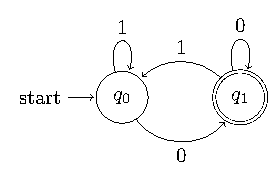
\includegraphics[width=0.75\textwidth]{figures/dfa.pdf}
\end{figure}



  


\section{Compilers}


Today's world undeniably relies on software more than ever before. It is imperative for developers to be able to efficiently write software. Software today is written in programming languages, high-level human-readable notations for defining how a program should run. However, before a program can be run on a system, it has to be translated (or compiled) into low-level machine code, which computers can run. The computer program that facilitates this translation is called a \emph{compiler}. See \cref{fig:compiler}.

\begin{figure}[h]
  \caption{Description of a compiler as a single unit.}
  \label{fig:compiler}
  \centering
  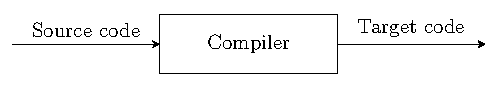
\includegraphics[width=0.75\textwidth]{figures/compiler.pdf}
\end{figure}



Compilers are complex programs. It is helpful to break them down into parts, each handling different tasks, which are chained together to form a compiler. Modern compilers are composed of many phases, such as the Lexical Analyzer, Syntax Analyzer, Semantic Analyzer, Intermediate Code Generator, Machine-Independent Code Optimizer, Code Generator, Machine-Dependent Code Optimizer \cite[p. 5]{dragon}, however this chapter covers the components relevant to this thesis. See relevant stages in \cref{fig:compiler-stages}.


\begin{figure}[h]
  \caption{Overview of relevant compiler stages.}
  \label{fig:compiler-stages}
  \centering
  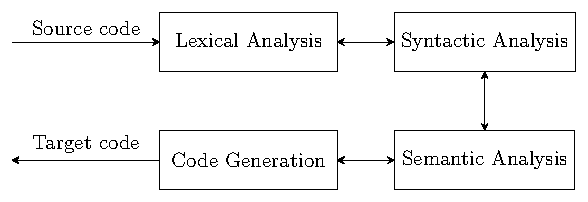
\includegraphics[width=0.75\textwidth]{figures/compiler-stages.pdf}
\end{figure}

\subsection*{Lexical Analysis}
The first stage of a compiler is lexical analysis, also known as a \emph{lexer} or \emph{tokenizer}. For the remainder of this thesis, \emph{lexer} will refer to the lexical analysis stage of a compiler. The lexer consumes a stream of characters, the \emph{source code}, and returns a stream of \emph{tokens}. A \emph{token} is a lexically indivisible unit, for example, the Python keyword \texttt{return}, you cannot divide it further, for example, into \texttt{re} \texttt{turn}. Each token is comprised of characters. The rule that defines which combination of characters constitutes a given token is called a \emph{pattern}. The sequence of characters matching a pattern is called a \emph{lexeme}, the \emph{lexeme} is stored along with the token as a value.

%Lexical analysis may be further divided into two distinct stages, however they are often implemented together. These stages are the \emph{scanner} and \emph{evaluator}.


\subsubsection*{Regular Expressions}
A compact way to represent the patterns accepting tokens are \emph{regular expressions}, which were introduced in \cref{def:regular_exp}. Regular expressions are an algebraic definition of patterns, they specify \emph{regular languages}, $\mathcal{L}_3$

\subsection*{Syntactic Analysis}

\subsubsection*{LL Parser}

\subsection*{Semantic Analysis}

\subsection*{Code Generation}


\chapter{Transpiler Implementation}
\section{Tools \todo{rename}}
\todo{mention python, sphinx, pytest, explain motivation for implementation of own transpiler}

\todo{mention lexer regex implementation}
\todo{mention LL table calculation according to theory}
\todo{write about transformation of ast}


\chapter{Evaluation of Results}
\todo{talk about methodology}
\todo{test examples analyticall vs FDTD}
\chapter{Conclusion}
\todo{compare lumerical and meep}
\todo{test result TBD}




%=========================================================================

% For compilation piecewise (see projekt.tex), it is necessary to uncomment it
% \end{document}
